% Chapter 1
\chapter{Introduction}
% Write in your own chapter title\label{Chapter 1}
\lhead{Chapter 1. \emph{Introduction}}
 % Write in your own chapter title to set the page header
%\section{Data mining}
 %
Data mining is the process for finding interesting and useful patterns from a dataset. The very first approach was finding frequent items i.e. the items that are used frequently. It plays an important role for finding knowledge discovery technique such as association rule mining, classification, clustering, time-series mining, graph mining, web mining etc. A lots of research and algorithm have been proposed for finding frequent patterns using Apriori based algorithms[], FP tree based algorithms[] and others algorithms[]. In real life, frequent item set finding application is used in market basket analysis \cite{agrawal1993mining}, medical image processing \cite{antonie2001application}, biological data analysis \cite{cong2004farmer} etc. Traditionally, all items in a transaction are treated equally. Though all items interest/influence is not same, they should be treated differently. For solving this problem, the notion of weighted item set mining has been introduced \cite{sun2008mining},\cite{tao2003weighted},\cite{wang2000efficient}. The weight of an item is the value that signifies the local interest within each transaction. 
\par
Several approaches have been proposed for IWIM (Infrequent Weighted Itemset Mining) \cite{manning2005new}, \cite{manning2008recursive}. In those approaches, they consider all data from the very beginning of the database. Therefore these approaches cannot be applicable for a large-scale data set such as data streams \cite{chang2005estwin}-\cite{chi2004moment},\cite{raissi2007towards}-\cite{leung2006dstree}, where data set flows in the form of continuous stream. Data stream is a continuous, unbound and ordered sequence of items that comes in order of time. In this case, it is impossible to maintain all data from the dataset and cannot possible to process all data at a time.  
\par
Existing algorithm works on whole fixed dataset and generates infrequent item set. For data stream, it have handle data in an efficient manner. Older data will be lost and also new updated data have to process. So it should differentiate recently generated data from older information which may unimportant or obsolete in context of time.
\par
Consider as an example, the data set in Table~\ref{tab:Table} where there is a set of transactions from data stream. Here we have considered a small part of the data set for simplicity. It contains eight transactions. These transactions are identified by tids. Each transaction contains four distinct items with their weights. It’s not necessary to be exact four items. Weight is defined by the corresponding degree of interest in the transaction i.e. item {\it b} contains weight 43 in tid 2 but in tid 3 is 0. Item weight is the value of CPU usage readings at a specific time. For data stream, this CPU usage reading is done at a fixed sampling rate. This CPU usage is important for data center resource management and application specific profiling. In tid4, weight of item {\it a} is 100. It means CPU a is working at high usage rate. While in tid 1, its weight is 0. It means temporarily {\it a} is idle. Knowledge extracting from this data set is important for domain expert or specific application expert to allocate system task break down for all CPU at a specific time.  So that, the system output can be maximized.
%

\begin{table}
\begin{center}
\begin{tabular}{ |c|c| } 
\hline
Transaction IDs (tid) & CPU usage reading \\
\hline
1 & (a,0) (b,100) (c,57) (d,71)\\
2 & (a,0) (b,43) (c,29) (d,71)\\
3 & (a,43) (b,0) (c,43) (d,43)\\
4 & (a,100) (b,0) (c,43) (d,100)\\
5 & (a,86) (b,71) (c,57) (d,71)\\
6 & (a,57) (b,71) (c,0) (d,71)\\
7 & (a,91) (b,32) (c,11) (d,0)\\
8 & (a,17) (b,61) (c,0) (d,72)\\
\hline
\end{tabular}
\caption{Example of a transaction data stream with weight}
\label{tab:Table}
\end{center}
\end{table}


\section{Basic Concepts}
 %
The main approaches of data mining include:\\
\textbf{Apriori:}
Apriori is a common approach for finding frequent items and association rule learning over transactional database. It was proposed by Agarwal and shrikant 1994[]. Apriori uses bottom-up approach. 
Subsets are extended one item at a time (also known as candidate generations) and groups of candidates are tested against the data. This procedure terminates when no further successful extensions 
are found. It uses breadth-first-search and a Hash tree structure to count candidate item sets efficiently. It generates candidate item sets of length K from item sets of length k-1. Infrequent 
sub patterns are pruned. Pruning is done based on minimum support $(min\_sup)$. Given a set of transactions (similar to database records in this context), where each transaction consists of
items (or attributes), an association rule is an implication of the form $A\Rightarrow B$, where A and B are sets of items and $A \cap B = \emptyset$. The support of this rule is defined as the percentage of transactions 
that contain the set $A \cup B$, while its confidence is the percentage of these ‘A’ transactions that also contain items in ‘B’. In association rule mining, all items with support higher than a 
specified minimum support are called frequent itemsets. One drawback of this approach is it requires multiple database scan. If number of items is large, it creates a lots of candidate patterns. 
It is also a limitation. \\
%
\textbf{FP Growth (Frequent Pattern Growth):}
FP-Growth algorithm was proposed by Han[]. It is an efficient way for finding frequent items without generating candidate list. It uses divide-and-conquer approach. It uses a special data structure 
named frequent pattern tree, which retains the itemset association information. It decomposes the mining task into a set of smaller tasks for mining confined patterns in conditional databases, 
which dramatically reduces the search space. FP-growth method is efficient and scalable for mining both long and short frequent patterns, and is about an order of magnitude faster than the Apriori 
algorithm and also faster than some recently reported new frequent pattern mining methods.\\

\textbf{Association Rule:}
Association rule is implied for discovering interesting relationships between variables in large databases. Following the original definition by Agrawal et al., [] The problem of association rule mining is defined as: 
Let {\it I} = \{{\it $i_1$, $i_2$, . . . . . . , $i_n$}\} be a set of n binary attributes called items.
Let {\it D} =\{{\it $t_1$, $t_2$, $t_3$,. . . . . ,$t_n$}\} be a set of transactions called the database. 
Each transaction in \textit{D} has a unique transaction ID and contains a subset of the items in \textit{I}.
A rule is defined as an implication of the form:
$X\Rightarrow Y$
Where $X,Y\subseteq I$ and $X \cap Y = \emptyset$ .
Every rule is composed by two different set of items, also known as itemsets, X and Y, where X is called antecedent or left-hand-side (LHS) and Y consequent or right-hand-side (RHS).\\

\begin{table}[h]
\begin{center}
\begin{tabular}{ |c|c|c|c|c|c| } 
\hline
Transaction IDs (tid) & milk & bread & butter & beer & diapers \\
\hline
1 & 1 & 1 & 0 & 0 & 0 \\
2 & 0 & 0 & 1 & 0 & 0\\
3 & 0 & 0 & 0 & 1 & 1\\
4 & 1 & 1 & 1 & 0 & 0\\
5 & 0 & 1 & 0 & 0 & 0\\
\hline
\end{tabular}
\caption{Sample transaction database}
\label{tab:Table14}
\end{center}
\end{table}

To illustrate the concepts, we use a small example from the supermarket domain in Table~\ref{tab:Table14}. The set of items is \textit{I} = \{milk, bread, butter, beer, diapers\} and in the table is shown a small database containing the items, where, in each entry, the value 1 means the presence of the item in the corresponding transaction, and the value 0 represent the absence of an item in a that transaction.
An example rule for the supermarket could be $\{butter, bread\} \Rightarrow {milk}$ meaning that if butter and bread are bought, customers also buy milk.


\textbf{Classification:}
Classification is the problem of identifying to which of a set of categories a new data belongs. It is done on the basis of a training set of data whose class label is known.\\
%
\textbf{Cluster Analysis:}
Cluster analysis deals with data for which the class labels are not known. Here, data is clustered or grouped based on the principle of maximizing the intraclass similarity and minimizing the interclass similarity \cite{book}. \\
%
\textbf{Outlier Analysis:}
A data set may contain some data which behaves differently than the rest of the data. This type of data is known as outlier. Sometimes this outliers provides us with useful information about the dataset. Analysis of these outlier data is known as outlier analysis.  
%
\section{Infrequent Itemset Mining} \label{sec:graph_mining}
%
Frequent itemset mining is a very common approach for finding frequent items. In our approach, we are trying to find infrequent items. Those  are the infrequent items, whose value is below threshold. For a given max{\_}support value, items value is below the max{\_}support. Infrequent item is important for resource management, application profiling, and fraud detection. It can be used for finding any unexpected or abnormal behaviour of a system. 

%
%\begin{figure}[ht]
%\centering
%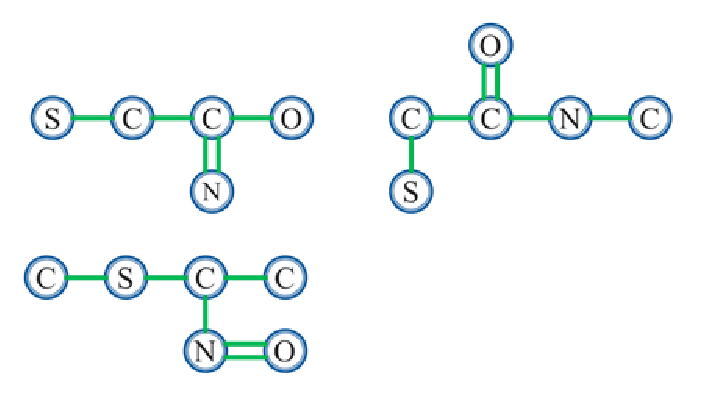
\includegraphics[scale = 0.8] {graph_data.eps}
%\caption{a set of chemical compounds represented using graph}
%\label{fig:graphdata}
%\end{figure} 
%
%



\section{Motivation}
%
Mining for infrequent itemset is recently gained attention of research community. Main focus for finding infrequent itemset whose frequency value is below \texttt{max\_support}. Not only frequency, weight can be also used for finding infrequent itemset mining. \\

\par
Let’s consider a scenario. A banking system where lots of transactions is done every day. As a bank officer, one may want to know if everything okay or not. In general cases, all transactions are okay but in fraud cases or unexpected cases, it may vary. It’s difficult for a bank officer to browse all data of the transactions to find any abnormal cases every day. It’s pretty hard for him. \\
\iffalse
%
\par \textbf{Motivating scenario:} \\
An application domain of graph classification related to the context of Bangladesh is drug discovery. Drug design and discovery is a growing field of interest in Bangladesh. The goal in drug discovery is to analyze this huge chemical space and identify molecules that show a certain desired activity. However, given the magnitude of the chemical space, an exhaustive exploration is not feasible \cite{drug}. Graph classification can be effectively used in this domain for molecular classification. \\
%
%\par The main goal of a graph classification approach is to classify graphs accurately and efficiently. But if we see some of the existing works we will find that, \\
%

\begin{itemize}
\item GAIA \cite{gaia} is a graph classification approach that makes use of evolutionary computation for feature selection purpose. But, it selects features by assigning  a score to a subgraph by only considering its own occurrence in the positive/negative graphs, it does not consider any other parameters. For this reason, its performance in terms of accuracy is not sufficient.
%
\item D\&D \cite{dnd} is one of the latest works in the field of graph classification. It provides a diversified discriminative score based on edge cover probability to select features. However, its performance is still not at satisfactory level. There is scope of improvement in terms of accuracy and runtime.
\end{itemize}
%
The above mentioned lackings of the existing works motivate us to develop a better graph classification approach.
%
\fi
\section{Objective}
%
We have studied that the existing approaches are limited to some context. As a solution, we have to develop an algorithm that can overcome the limitations. The objectives of our work are listed below:
%
\begin{itemize}
\item To carry out an extensive literature view regarding the infrequent itemset mining approach.
\item Propose a new efficient algorithm for finding infrequent items. 
\item Propose an algorithm that can perform in broader area.
\end{itemize}
%
\section{Thesis Contribution}
%
The contributions our research work are listed below:
%
\begin{itemize}
%
\item We have used sliding window based approach. This reduces the processing time \& memory space.
%
\item We can get the actual contribution of an item in the dataset. Previous approach uses equivalence weighting function for data items.
% 
\item It’s easier to discard frequent items from the candidate infrequent pattern list.
\item Extra cost for checking infrequent patterns validation (i.e. is the item actually infrequent or not) is not required.
%
\end{itemize}
%
\section{Thesis Outline}
The five chapters labeled as Introduction, Related Work, Proposed Approach, Performance Evaluation and Conclusion form the shape of the book.
Every chapter comprises of the following topics: \\
%
Chapter 1 contains some introductory concepts such as data mining and various data mining approaches, infrequent itemset mining and also the motivation and contribution of this work.\\
%
Chapter 2 describes various terms related to previous work in the field of infrequent itemset mining and also the limitations of the existing approaches. \\
%
Chapter 3 describes the proposed score and algorithm. It also contains the details of our work and application of the proposed algorithm. \\
%
Chapter 4 contains the implementation results and performance evaluation results of the proposed algorithm. \\
%
Chapter 5 draws the conclusion of the thesis by summarizing the
findings in the thesis and describing scope of possible extensions to this work. \\
%
The last part of the book is Bibliography which places all the reference cited in the work. The appendix works as additional information that helps the reader if necessary.
%
